\documentclass[12pt]{article}
%\documentclass[paper=a4]{scrartcl}
\usepackage{ucs}     % unicode 
\usepackage[utf8x]{inputenc}  % utf-8
\usepackage[ngerman]{babel}  % new german spelling 
\usepackage{graphicx}   % use graphics 
\usepackage{fancyhdr}   % header and footer
%\usepackage{scrpage2} 
\usepackage{setspace}
\usepackage{url}
\usepackage{tikz}
\usepackage{tikz-qtree}
\usepackage[printonlyused]{acronym}
\usepackage{a4wide} %depricated, use: geometry 
%\usepackage{cite}
\usepackage{natbib}	% bibstyle 
\usepackage[section]{placeins}	% \FloatBarrier
\usepackage[T1]{fontenc} %enable hyphenation for words including umlaute
\usepackage[pdfborder={0 0 0}]{hyperref} %links, aber ohne Rahmen
\usepackage{nameref} %Verweise auf sections
\usepackage{amsmath}

% Settings
\hyphenation{TIGER} % do not hyphenize
\bibpunct{[}{]}{,}{a}{}{;}


\setcounter{tocdepth}{2}
\begin{document}

\thispagestyle{empty} 

\begin{center}
	\topskip0pt
	\vspace*{\fill}
	
	\Huge{\textbf{Seminararbeit}}\\
	\vspace{1.5cm}
	
	\Large{\textbf{Automatische Bestimmung semantischer Rollen im deutschen
	Korpus SALSA 2.0}}\\
	\vspace{1cm}
		
	
\includegraphics[scale=0.3]{images/logo_hu.png}
	\vspace{1cm}

	\begin{Large}
		Institut für Informatik \& Institut für Linguistik\\
		Humboldt-Universität zu Berlin\\
		\vspace{1.5cm}
		Robert Bärhold \& Arne Binder \\
		31. März 2014 \\ %TODO
		\vspace{1cm}
		
		\begin{table}[h]
			\Large
			\centering
			\begin{tabular}{l l}
				Seminar: & Computergestützte Analyse von Sprache\\
				Seminarleiter: & Prof. Dr. Ulf Leser\\
				 		    & Prof. Dr. Anke Lüdeling \\
				Semester: & Wintersemester 2013/14 				 	
			\end{tabular}
		\end{table}	
	\end{Large}
	\vspace*{\fill}
\end{center}


\pagenumbering{roman}
\pagestyle{fancy} %eigener Seitenstil
\fancyhf{} %alle Kopf- und Fußzeilenfelder bereinigen
\renewcommand{\headrulewidth}{0pt} %obere Trennlinie
\renewcommand{\footrulewidth}{0pt} %untere Trennlinie 
\fancyfoot[C]{\thepage} %Seitennummer

 \newpage
 \tableofcontents
 \vspace{1cm}
 \listoffigures
 \vspace{1cm}
 \listoftables

\newpage
\pagenumbering{arabic}

\section{Einleitung}
- warum SRL? Motivation
- was gibt es schon? related work
[Shalmaneser, gildea \& jurafski, SEMAFOR, LTH, ...]
\subsection{Semantische Rollen}

Prädikate zeichnen sich dadurch aus, dass sie die Komplementationsstruktur einer
übergeordneten syntaktischen Einheit (nämlich des Satzes) bestimmen. Zum
Beispiel verlangt ein ditransitives Verb wie \glqq{}geben\grqq{} drei weitere Satzkonstituenten mit konkreten syntaktischen Eigenschaften:

\begin{center}
	\begin{tikzpicture}
		\Tree [.geben
				[.Subjekt Paul ]
				[.{} gibt ]
				[.Akk-Objekt {die Jacke} ]
				[.Dativ-Objekt {seiner Freundin} ]
			]
			
		%\Tree [.geben
		%		[.\textbf{Subjekt} Paul ]
		%		[.{} gibt ]
		%		[.\textbf{Akk-Objekt} {die Jacke} ]
		%		[.\textbf{Dativ-Objekt} {seiner Freundin} ]
		%	]
	\end{tikzpicture}
\end{center}

Aber das Bedingtheitsverhältnis zwischen dem Verb und seinen Komplementen 
endet nicht in der Syntax. Diese sind durch das Prädikat auch hinsichtlich ihrer 
\textit{semantischen} Integrierung in den Satz determiniert. Dem Komplement \glqq{}Paul\grqq{}
wird einmal die syntaktische Funktion des Subjekts zugewiesen, es wird aber auch
durch die konkrete Semantik der Handlung \glqq{}geben\grqq{} als 
\glqq{}Geber\grqq{} charakterisiert. Man spricht von den Argumenten
eines Verbs und sagt, dass sie \textit{semantische Rollen} realisieren. So realisiert \glqq{}Paul\grqq{} im obigen Beispiel die semantische Rolle \glqq{}Geber\grqq{}.

\subsection{Frame Semantik}

Die traditionelle Semantik [TODO: evtl. welche traditionelle Sem.? Referenz?] war versucht, eine möglichst abstrakte und
allgemeine, intersprachliche Formulierung von semantischen Rollen zu
finden - bei der man z. B. nicht von \glqq{}Geber\grqq{} sondern allgemein
von \glqq{}Agens\grqq{} sprechen würde. Demgegenüber steht die von C.J. Fillmore
ab den 70er Jahren entwickelte Theorie der Frame-Semantik (FS)
[\cite{fillmore1985}]. Das Fundament der Theorie ist mit dem traditionellen
Ansatz in höchstem Maße inkompatibel, für unser Vorhaben reicht es aber, die
partikuläre Auffassung von semantischen Rollen zu erwähnen, die der
Frame-semantische Ansatz mit sich bringt.

Rollen bzw. Frame-Elemente (FE) in Termini der FS werden nicht in Bezug auf die
Argumentstruktur von Verben formuliert, sondern hinsichtlich der globalen
Situation (oder des \textit{Frames}), die durch das Prädikat evoziert wird. Aufgrund
des situationellen Charakters der Frames sind nicht nur Verben sondern auch
Nomina (\textit{Mord}, \textit{Auge}\footnote{beispielsweise als Indikator für ein Ereignis der Wahrnehmung: \glqq{}Vor seinen Augen zerrissen sie die Bücher.\grqq{}}, \textit{Frau} von jemandem) oder Adjektive (\textit{stolz} auf etwas sein) potentielle
Frame-einführende Elemente, und in diesem Sinne auch Prädikate. Nachfolgend ist der Frame \glqq{}Kritik1-salsa\grqq{} dargestellt, so wie er im framesemantisch-annotierten SALSA 2.0 Korpus [\cite{rehbein_adding_2012}] definiert ist:

\begin{quote}
\textbf{Definition:}
A Reviewer offers his or her assessment of a work of art or performance (e.g. a play, a novel, a piece of music composition etc). The Reviewer typically bases his judgment on their own expertise and uses some set of criteria for evaluating works as to their relative merit.

\textbf{Example Sentences:}
\begin{enumerate}
\item Ich hab absichtlich auch noch keine anderen \textbf{Kritiken} gelesen und möglicherweise hab ich ein paar Dinge in dem Film übersehen.
\item Ich bin auf das Buch durch die \lbrack lobende\rbrack \textsuperscript{Valence} \textbf{Kritik} \lbrack in der FAZ\rbrack \textsuperscript{Medium} aufmerksam geworden.
\item \lbrack Olaf Storbecks Jahrhundertkrise\rbrack\textsuperscript{Evaluee}\lbrack erntet\rbrack\textsuperscript{Support} erste\lbrack gute\rbrack \textsuperscript{Valence} \textbf{Kritiken}.
\item Star Dreck - \lbrack Negative\rbrack \textsuperscript{Valence} \textbf{Kritiken} \lbrack von Fans\rbrack \textsuperscript{Reviewer}  \lbrack zum neuen Star Trek\rbrack \textsuperscript{Evaluee}
\end{enumerate}


\textbf{FEs}


\textbf{FE1(Reviewer)}: The person assessing the Evaluee for its merit.

\textbf{FE2(Evaluee)}: The cultural artifact that is evaluated.

\textbf{FE3(Medium)}: The venue or publication in which the review is distributed.

\textbf{FE4(Valence)}: The positive or negative nature of the evaluation, if specified. 
\end{quote}

\subsection{Semantic Role Labeling}\label{subsec:introduction_SRL}

Mit Semantic Role Labeling (SRL) ist die automatisierte Erkennung und
Annotierung von semantischen Rollen innerhalb eines Satzes gemeint. Die primäre
Aufgabe von SRL ist die genaue Identifizierung der semantischen Beziehung
zwischen einem Prädikat und seinen assoziierten Elementen und Eigenschaften
(siehe \cite{SRL2008} für eine allgemeine Darstellung). In Bezug auf eine FS lässt
sich folgendes feststellen. Da FE Frame-spezifisch sind, stellen sie eine
Zwischenstufe in der semantischen Abstraktion zwischen der rein lexikalischen
Bedeutung und den traditionellen Verbenübergreifenden [@Enrique: was meinst hier mit Verb..übergr.?] semantischen Rollen dar.
Die dadurch erreichte \glqq{}mildere\grqq{} Stufe der Abstraktion über die
Rollen der verschiedenen Verben, Nomina und Adjektive eignet sich besonders gut
für die Lösung unterschiedlicher Aufgabenstellungen in Bereichen des
Sprachverstehens [TODO: Leser konnte hiermit nichts anfangen :-( kann man das irgendwie erläutern/konkretisieren?] wie der Informationsextraktion oder Dialogsystemen [TODO: Verweis/Erklärung]. [\cite{gildea}]

[TODO kürzen und einbauen(an richtiger Stelle): The relationship between such surface manifestations and
semantic roles is the subject of linking theory—see \cite{levinrappaport}
for a synthesis of work in this area. In general, linking theory argues that the syntactic
realization of arguments of a predicate is predictable from semantics—exactly how this
relationship works is the subject of much debate. Regardless of the underlying mechanisms
used to generate syntax from semantics, the relationship between the two suggests
that it may be possible to learn to recognize semantic relationships from syntactic
cues, given examples with both types of information.]

Die Aufgabenstellung eines FS-orientierten SRL-Systems lässt sich im Allgemeinen
wie folgt untergliedern:
\begin{enumerate}
\item Zunächst wird der Frame, der durch den Satz oder die Phrase realisiert wird, bestimmt.
\item Es folgt die Bestimmung der Frame-Elemente bezüglich des Frames. 
\item Schließlich erfolgt die Klassifizierung der einzelnen Frame-Elemente.
\end{enumerate}


\section{Problemstellung}
Im Zuge dieser Arbeit soll die Frage geklärt werden, ob sich der Ansatz von \cite{gildea} auf einer Baumbank, das heißt einem Phrasen-annotierten Textkorpus, der deutschen Sprache adaptieren lässt. Dieser Ansatz besagt, dass mithilfe lexikalischer und syntaktischer Informationen verlässliche Annahmen über die Realisierung von semantischen Rollen durch Konstituenten eines Satzes getroffen werden können. Die Annahme lässt sich dazu nutzen, ein automatisiertes, statistisches Lernverfahren basierend auf einem zusätzlich mit Rollen annotierten Korpus zu entwickeln, welches die automatische Bestimmung der in einem deutschen Satz realisierten semantischen Rollen mit akzeptabler Genauigkeit ermöglicht.

\subsection{Korpus: Salsa 2.0}
Grundlage dieser Arbeit bildet das SALSA Korpus in der Version 2.0. Das SALSA Korpus ist ein für akademische Zwecke frei zugängliches, framesemantisch annotiertes Korpus der deutschen Sprache. Es basiert auf TIGER\citep{brants_tiger_2002, tiger}, einer Baumbank aus deutschen Zeitungsartikeln, welche semi-automatisch mit POS-Tags, Lemma-Informationen und syntaktischen Strukturen annotiert wurde.\footnote{Für weitere Informationen siehe \url{http://www.ims.uni-stuttgart.de/forschung/ressourcen/korpora/tiger.html}.}

SALSA erweitert TIGER um semantische Informationen. Jedem Satz sind ein oder mehrere Frames zugeordnet. Ein Frame besteht aus einem Target, das ist das Prädikat, das den Frame evoziert, und verschiedenen Frame-Elementen, also den Elementen des Satzes, die eine semantische Rolle innerhalb des Frames realisieren. Frame und Frame-Elemente werden innerhalb des Korpus durch einen Namen und eine eindeutige ID charakterisiert, dem Target ist lediglich das zugehörige Lemma zugewiesen. Sowohl das Target als auch die Frame-Elemente können aus mehreren Konstituenten bestehen.

Der Großteil der Frames wurde vom englischsprachigen FrameNet-Projekt\citep{baker_berkeley_1998} übernommen.\footnote{Für weitere Informationen siehe \url{https://framenet.icsi.berkeley.edu/fndrupal/}.} Diese wurden um einige deutschsprachliche Frames ergänzt. Einzelne Frames und auch Frame-Elemente sind über verschiedenste Relationen miteinander verknüpft. Durch solche Relationen werden beispielsweise Hyperonomie, Meronymie, Synonymie sowie kausative Zusammenhänge abgebildet.
%Hyperonomie: Oberbegriff # Meronymie: Teil-Ganzes-Beziehung

Die Version 1.0 des SALSA Korpus\citep{burchardt_salsa_2006} enthält Frames dessen Targets ausschließlich Verben sind. Mit der Weiterentwicklung zur Version SALSA 2.0\citep{rehbein_adding_2012} sind außerdem durch Nomen realisierte Prädikate und deren zugehörige Frames annotiert worden. Das SALSA Korpus 2.0 besteht aus circa 24.000 Sätzen. Es enthält rund 20.000 verbale und mehr als 17.000 nominale Instanzen, welche durch 648 verschiedene Targets ausgelöst werden.

\section{Realisierung des SRL-Klassifikators}
In diesem Abschnitt wird die Realisierung des entwickelten Klassifikators zur automatischen Annotation von semantischen Rollen genauer beschrieben. Hierfür werden zunächst die getroffenen Annahmen dargelegt. Im Anschluss werden die von \cite{gildea} adaptierten sowie zusätzlich verwendete Features erläutert. Abschließend wird die Arbeitsweise des Klassifikators veranschaulicht.

\subsection{Annahmen}

Analog zu \cite{gildea} wurde die Annahme verfolgt, dass gleiche Rollen auch in verschiedenen Frames ähnlich morphosyntaktisch realisiert werden. Es werden daher nur die im Frame enthaltenen Frame-Elemente als relevante Informationsträger betrachtet - unabhängig vom einbettenden Frame. Eine Disambiguierung der verschiedenen Frames, die durch das selbe Prädikat evoziert werden, ist daher nicht möglich. Bezogen auf die Trainingsdaten entfällt somit eine Abstraktionsebene, so dass die nur sehr spärlich zur Verfügung stehenden Trainingsdaten\footnote{Für den Gesamtkorpus gilt: es gibt pro FE durchschnittlich 100 Instanzen} besser ausgeschöpft werden können.

Im Hinblick auf den in Abschnitt\ref{subsec:introduction_SRL} vorgestellten allgemeinen SRL-Prozess entfällt der erste Schritt. Die Schritte zwei und drei werden im Unterschied zu \cite{gildea} in einem Zug durchgeführt, da ein kompaktes automatisiertes Lernverfahren in der Regel qualitativ besser abschneidet als hintereinandergeschaltete Teilsysteme.

Da einzelne syntaktische Features nur im Bezug zu einem Target existieren und aus Gründen der Komplexität keine Abstraktion auf ungesehene Targets vorgenommen wird, wurde einschränkend festgelegt, dass das Target bekannt sein muss.

\subsection{Features}
Die genutzten lexikalischen und syntaktischen Features sind, bis auf das Feature \textit{Nachbar-Kopf-Lemma}, ebenfalls stark an \cite{gildea} orientiert. Sie werden für jede atomare sowie komplexe Konstituente (Phrase) extrahiert.

[TODO: kein voice-feature]


\subsubsection*{Syntaktische Kategorie}
Für komplexe Konstituenten entspricht dieses Feature der phrasalen Kategorie, bei atomaren Konstituenten wird das POS-Tag genutzt.
\subsubsection*{Pfad}
Eines der wichtigsten syntaktischen Features wird aus dem Pfad zwischen der aktuell betrachteten Konstituente und der Target-Konstituente innerhalb des Konstituentenbaums gebildet. Er setzt sich aus den verschiedenen Phrasenkategorien der dazwischenliegen komplexen Konstituenten zusammen. Die einzelnen Kategorien werden mit einem Richtungsmarker (absteigend oder aufsteigend im Baum) verknüpft. Um die Anzahl der Werte dieses Features etwas zu minimieren, werden direkte Wiederholungen einer gleichen Phrasenkategorie zusammengefasst und koordinierende Phrasenkategorien nicht berücksichtigt.
\subsubsection*{Position}
Ein weiteres syntaktisches Features ist die Position der aktuell betrachteten Konstituente in Bezug zum Target. Es wird das Kopfelement der Konstituente betrachtet. Dieses kann vor einem atomaren Target (0), vor einem komplexen Target (1), innerhalb eines komplexen Targets (2) und nach einem Target (3) stehen.
\subsubsection*{Kopf-Lemma}
Als lexikalisches Feature wird das Kopfelement genutzt, also die atomare Konstituente, die den wichtigsten syntaktisch determinierenden Beitrag innerhalb einer komplexen Konstituente leistet. Außerdem leisten Kopfelemente den zur Problemlösung relevantesten semantischen Beitrag. Es wird die lemmatisierte Form des Wortes genutzt. Für atomare Konstituenten
wird die Konstituente selbst als Kopfelement gesetzt.

Da im TIGER-Korpus nicht für alle Typen phrasaler Konstituenten ein Kopfelement definiert ist\footnote{Nach Abschluss der Programmentwicklung hat sich herausgestellt, dass eine Konvertierung von TIGER in eine Dependenzgrammatik existiert [\cite{kountz_extraktion_2006}] und somit für den Großteil der Konstituenten eindeutige Kopfelemente gegeben wären.}, wird regelbasiert von der aktuellen Konstituente ausgehend Richtung ihrer Kinder nach einem Kopfelement gesucht, falls es nicht bekannt ist. Dabei werden die jeweiligen grammatikalischen Funktionen der Kind-Konstituenten sowie die Phrasenkategorien ausgewertet.\footnote{Die Label für die grammatische Funktion (Kanten-Label der Baumbank) und die der Phrasenkategorien folgen dem NEGRA-Tagset (siehe http://www.coli.uni-saarland.de/projects/sfb378/negra-corpus/negra-corpus.html).} Wenn die Suche auf eine Konstituente trifft, die atomar ist oder für die ein Kopf definiert ist, wird dessen Lemma als Kopfelement bis zum Ursprung der Suche Baum-aufwärts propagiert und dabei für alle Konstituenten auf diesem Pfad gesetzt. Köpfe sind somit immer atomar.
\subsubsection*{Target-Lemma}
Hierzu wird das Lemma des Kopfes der kleinsten Konstituente herangezogen, die alle Teile des Targets überdeckt.
\subsubsection*{Nachbar-Kopf-Lemma}
An Hand von Experimenten hat sich herausgestellt, dass der Kopf der kleinsten Konstituente, welche die aktuell betrachtete überdeckt und dessen Kopf außerhalb dieser liegt, relevante Informationen für die SRL-Klassifikation liefert.



\subsection{Arbeitsweise des Klassifikators}

Analog zu \cite{gildea} stellt ein Naïve-Bayes-Klassifikator die Grundlage der Implementierung dar. Wie bei statistischen Klassifikationsverfahren üblich, gliedert sich diese in eine Trainingsphase, also die Erstellung des Modells, und eine Klassifikationsphase, in der das eigentliche Semantic Role Labeling stattfindet. Die Vorteile des Naïve-Bayes-Klassifikators liegen in der Einfachheit und Transparenz der Funktionsweise. Die dem trainierten Modell inhärenten Wahrscheinlichkeitsverteilungen liefern meist auch vom Menschen leicht interpretierbare Informationen, welche bei der Entwicklung des Klassifikators und der Auswahl der Features sehr hilfreich waren. 



%\begin{align}
%P(r|c)&=P(r|f_1,...,f_n)\\
%&=\underbrace{P(r)}_{\approx \frac{\#(r)}{\#(all)}}\prod_{i=1}^n \underbrace{P(f_i|r)}_{\substack{=\frac{P(f_i\cap r)}{P(r)}\\\approx\frac{\#(f_i, r)}{\#(r)}}}\\
%log(P(r|c))&\approx log\left(\frac{\#(r)}{\#(all)}\right) + \sum_{i=1}^n log\left(\frac{\#(f_i, r)}{\#(r)}\right)
%\end{align}

\subsubsection*{Erstellung des Modells}
%- keine Frames über mehrere Sätze

Beiden Phasen ist gemein, dass das jeweils genutzte Korpus geparst und vorverarbeitet werden. Dabei werden für alle Konstituenten die Start- und Endpositionen im Satz und die Köpfe wie zuvor beschrieben bestimmt.


Da allerdings einige Beziehungen zwischen den einzelnen Features semantisch relevant sind, werden nicht immer rein naiv die Einzelwahrscheinlichkeiten multipliziert, sondern auch die Wahrscheinlichkeiten für bestimmte Feature-Kombinationen ermittelt[ und beim klassifizieren nachgeschlagen]. Nur Falls diese für die aktuell zu klassifizierende Konstituente im Modell nicht gefunden werden, kommen die Einzelwahrscheinlichkeiten zum Einsatz. So wird erneut der geringen Trainingsdatenmenge entgegengewirkt. Wann genau [durch dieses Back-Off-Modell] auf welche Einzelfeatures zurückgegriffen wird, ist im Abschnitt \nameref{subsubsec:classify} genauer erläutert.

\subsubsection*{Klassifikation der Konstituenten}\label{subsubsec:classify}
%keine Abstraktion für ungesehene Targets

Back-Off-Model

smoothing-value $= 10^{-6}$
\section{Evaluation des xxxxx} %TODO

Der entwickelte Ansatz der automatischen Rollenannotation wurde nach Abschluss
der Entwickelung einer Evaluation unterzogen. Diese sollte Aufschluss über die
Qualität der entwickelten Anwendung geben, so dass ein Vergleich mit ähnlichen
Systemen gezogen werden kann.

Abbildung \ref{featureImpact} verdeutlicht den Einfluss der verschiedenen Features. Die Werte geben die Abnahme der Prozentpunkte von F-Measure/Precision/Recall an, wenn das jeweilige Feature nicht genutzt wird. Die bedeutendsten Features sind der Pfad und das Nachbar-Kopf-Lemma. [TODO: Grafik übersetzen!]
\begin{figure}[Einfluss der Features]
			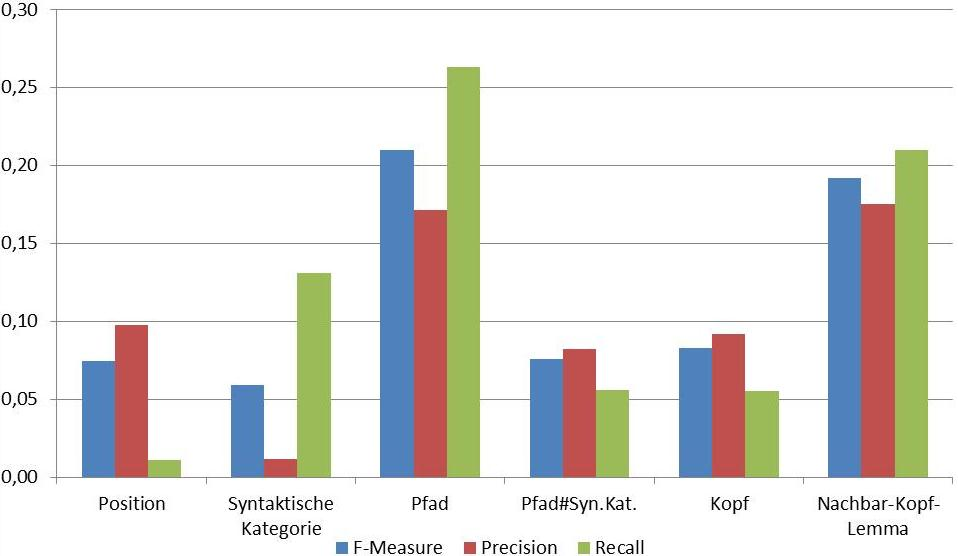
\includegraphics[scale=1.0]{images/featureImpact_sorted.jpg}
			\caption{Der Einfluss der Syntaktischen (Syntaktische Kategorie, Pfad \& das aus dem Pfad und der syntaktischen Kategorie zusammengesetzte Feature) und lexikalischen Features (Kopf-Lemma \& Nachbar-Kopf-Lemma)}
			\label{featureImpact}
\end{figure}


\newpage
\bibliography{biblio}
\bibliographystyle{natdin}


\end{document}